\subsection{Drift Chamber smearing}
The DC resolution must be properly incorporated in the MonteCarlo. The steps below describe this procedure.

When a particle passes throught a DC cell, see \F{fig:dc_cell}, the sensible wire signals a drift time, which is then turned 
into distance from the wire, or $CalcDoca$ (DOCA = distance of closest approach).

\begin{figure}[h]
 \begin{center}
 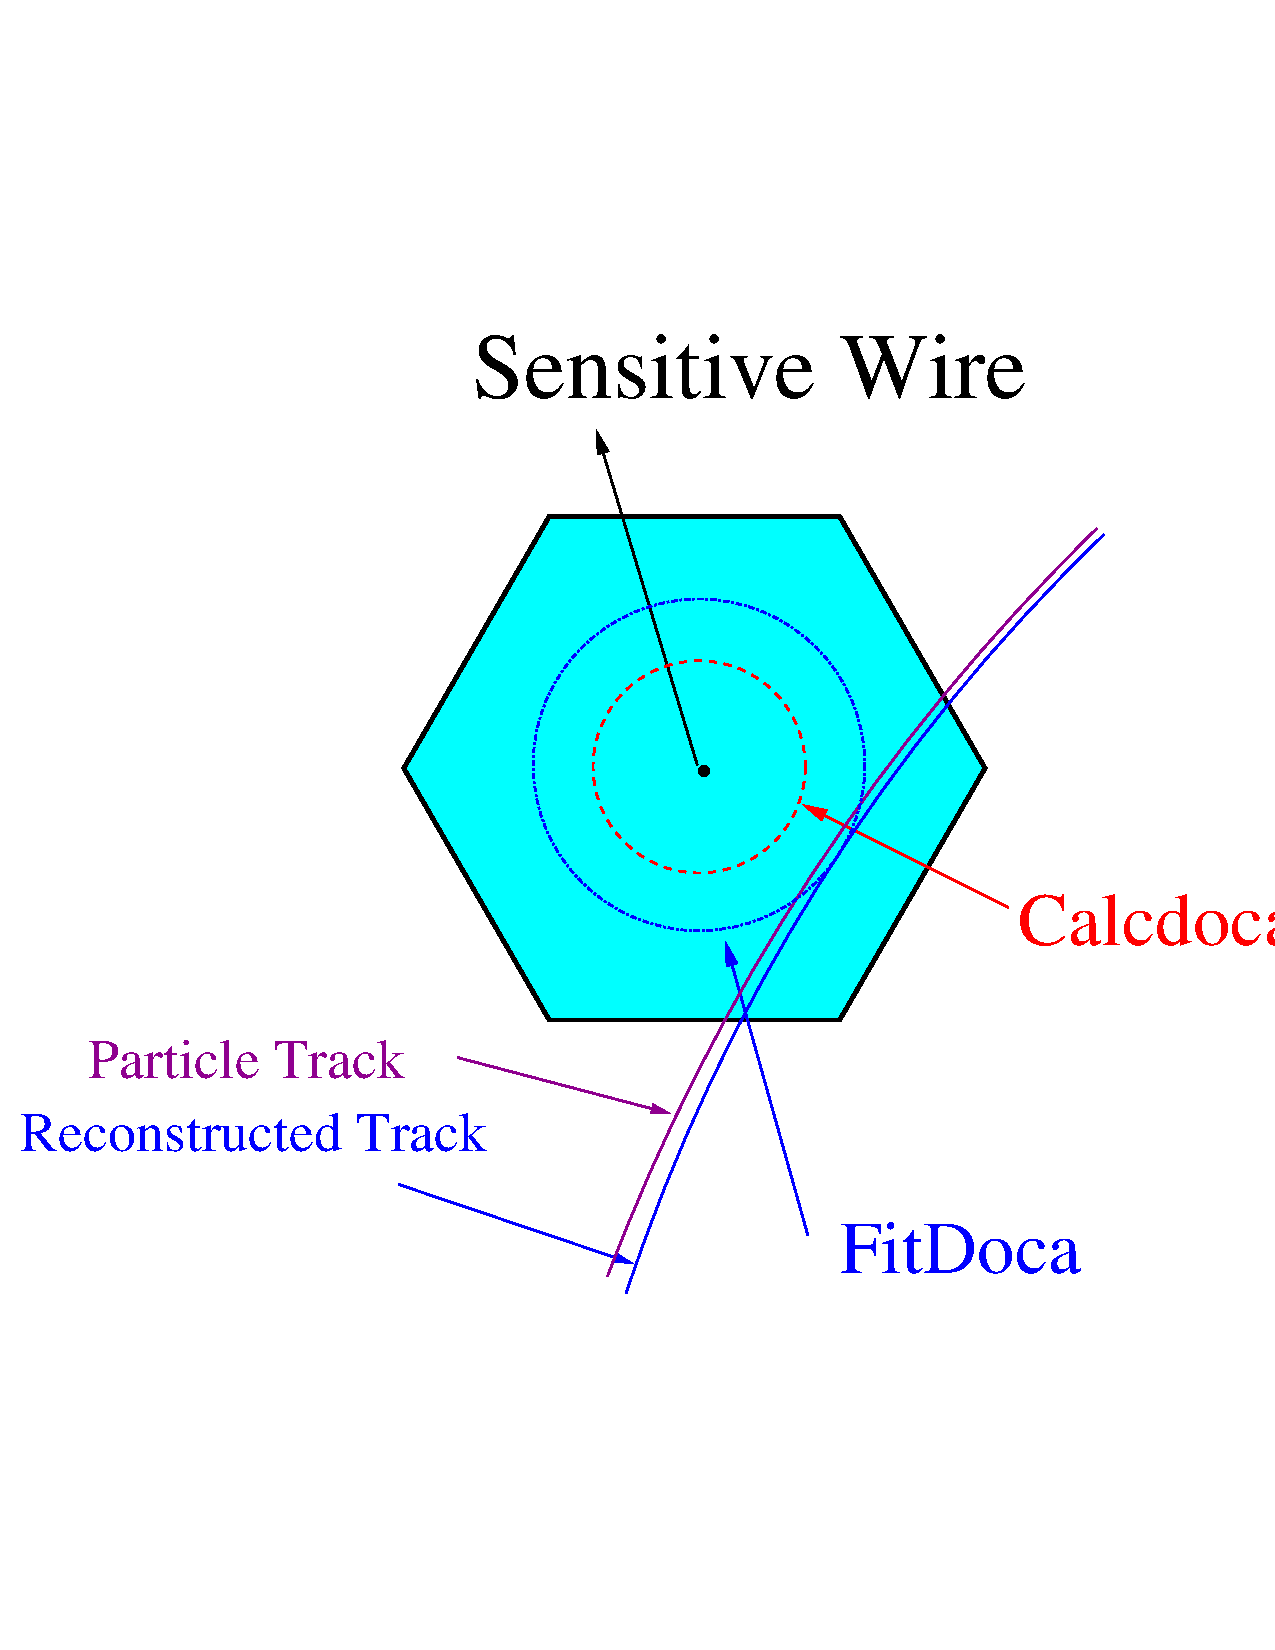
\includegraphics[width = 12cm, bb=-60 140 700 700]{acceptance/img/dc_cell} 
  \caption[A charged particle passing through a DC cell]
          { A charged particle passing through a DC cell. The drift time is converted into $CalcDoca$ which
	             is used by the tracking procedure to find the reconstructed track. The resulting distance
		     from the wire, or $FitDoca$, is much closer to the real track. }
 \label{fig:dc_cell}
 \end{center}
\end{figure}

During the tracking procedure the information from all the cells is taken into account so that the resulting
$FitDoca$, the distance of the wire from the reconstructed track,  will be much closer to the actual track.

The quantity 
\begin{equation}
SR = |CalcDoca| - |FitDoca|
\end{equation}
(called Spacial Residual) is a good estimate of the DC resolution because it measures
the response of a single cell.
This quantity 
is plotted against $FitDoca$ for the DC Region 3 in \F{fig:dc_res}. One can see that 
the  mean and the $\sigma$ of the distribution are not constant, however only the $\sigma$
can be incorporated in the MonteCarlo\footnote{The mean position comes 
from the convolution, which is unknown, of the actual position in the cell with the tracking procedure.
The $\sigma$ is not affected by this convolution.}.

\begin{figure}[h]
 \begin{center}
 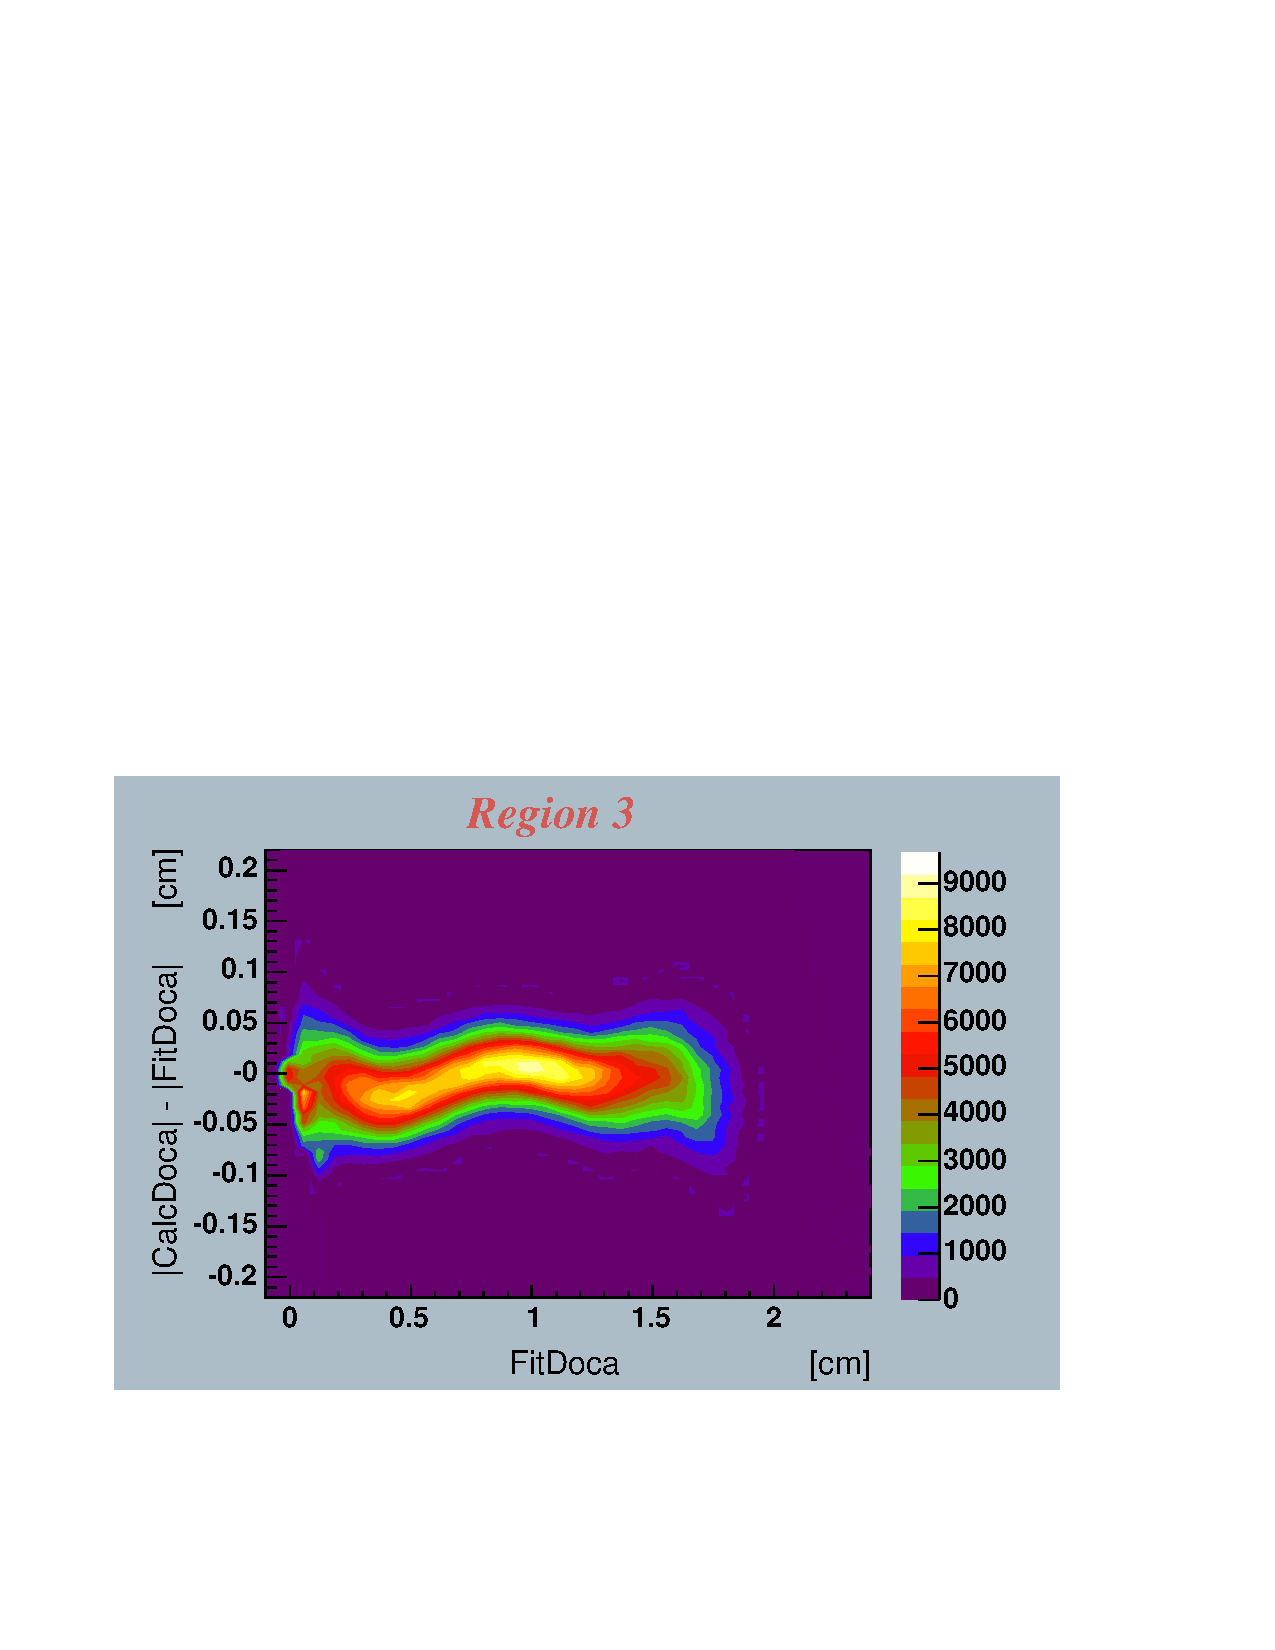
\includegraphics[width = 12cm, bb=50 100 600 450]{acceptance/img/re3} 
  \caption[The space residual for DC Region 3]
          { The space residual for DC Region 3. The mean and the $\sigma$ 
	             of the distribution are not constant. }
 \label{fig:dc_res}
 \end{center}
\end{figure}


The distribution in \F{fig:dc_res} is sliced along the $y-axis$ and each slice is fitted with 
a gaussian distribution. The result is plotted in \F{fig:dc_sigma}, where a fit is performed.
This procedure is applied for each region of the DC. It was found that the sector or superlayer
dependance of the $\sigma$ distribution is negligible. 
The parameters of the fit in \F{fig:dc_sigma} are incorporated in the MonteCarlo (by mean of a mysql database).

\cia
In \F{fig:dc_sigma_comp} is shown the comparison of real data (black) and 
the obtained MonteCarlo (red) DC resolution for Region 2. The simulated and true 
data shows good agreement.

\begin{figure}[h]
 \begin{center}
 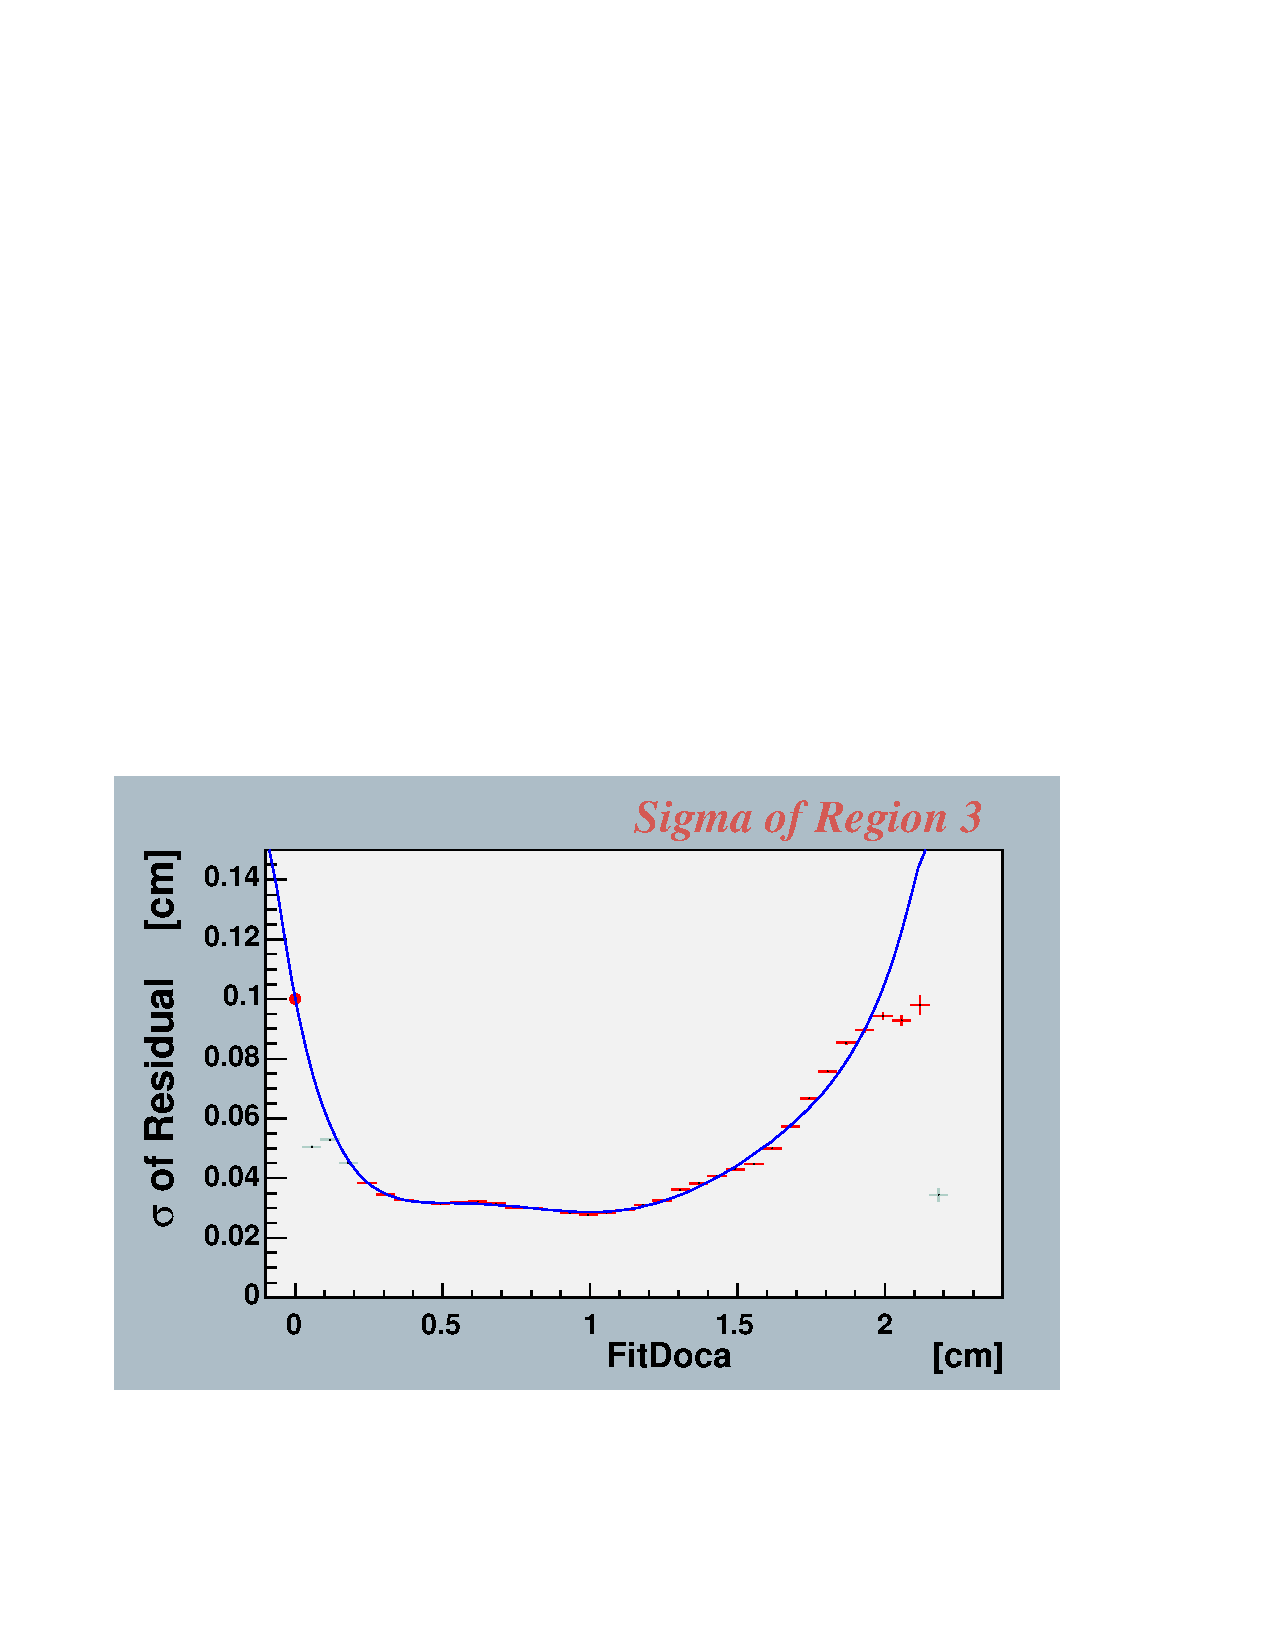
\includegraphics[width = 12cm, bb=0 100 620 450]{acceptance/img/res3} 
  \caption[The $\sigma$ of the space residual for DC Region 3]
          { The $\sigma$ of the space residual for DC Region 3. The parameters of the fit are
	             incorporated in the MonteCarlo (by mean of a mysql database).}
 \label{fig:dc_sigma}
 \end{center}
\end{figure}




\begin{figure}[h]
 \begin{center}
 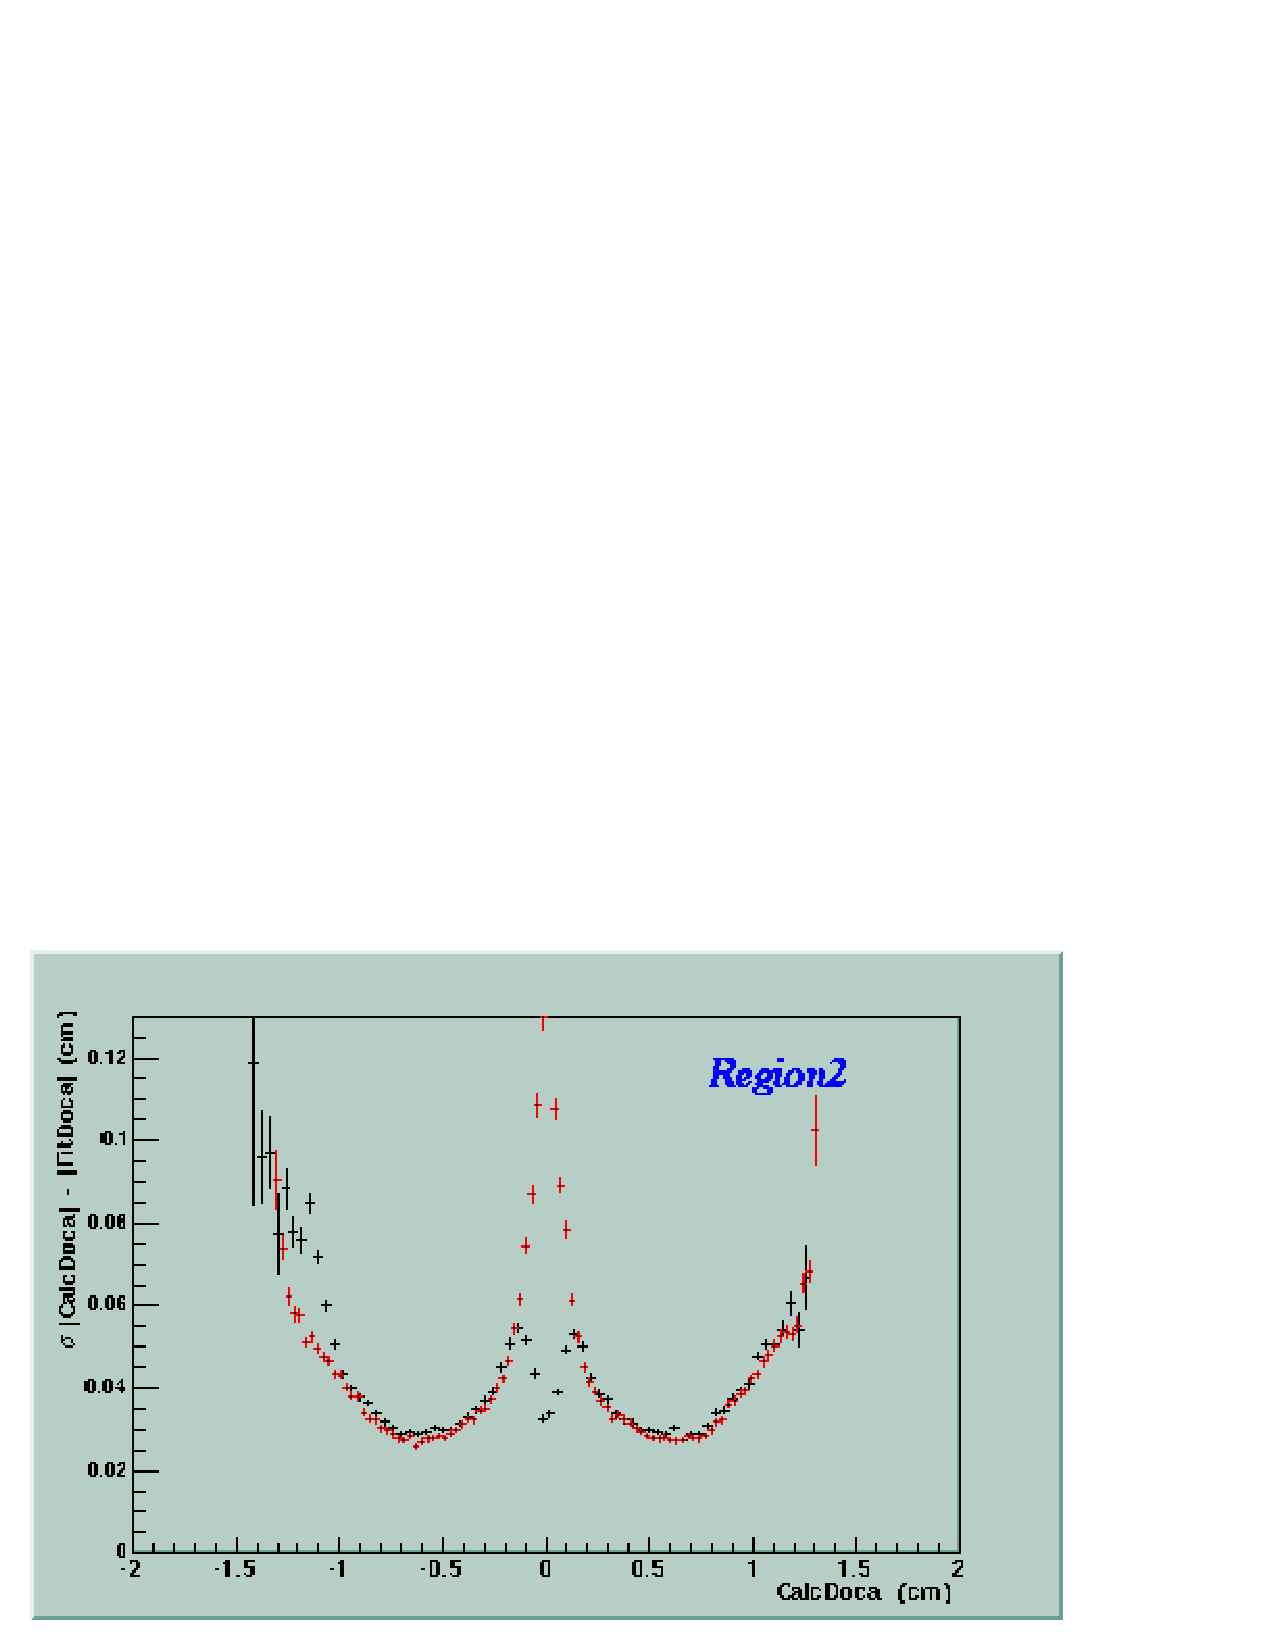
\includegraphics[width = 12cm, bb=-30 0 620 350]{acceptance/img/reg2r} 
  \caption[Comparison of real data and MonteCarlo DC resolution for Region 2.]
          { Comparison of real data (black) and MonteCarlo (red) DC resolution for Region 2.
	             The difference at $FitDoca\sim 0$ is due to the fact that the residual for the MonteCarlo
		     is calculated before tracking (it is in fact the actual resolution of the cells).}
 \label{fig:dc_sigma_comp}
 \end{center}
\end{figure}




